\documentclass[onecolumn]{IEEEtran}

\usepackage{algorithm,algpseudocode}
\usepackage{amsmath}
\usepackage{array}
\usepackage{authblk}
\usepackage{caption}
\usepackage[utf8]{inputenc}
\usepackage{mathtools}
\usepackage{nameref}
\usepackage{graphicx}
% \graphicspath{ {images/} }

% metadata
\author{Ricardo Soto Estévez}
\affil{Menendez Pelayo International University}
\date{\today}
\title{Practical study of basic Genetic Algorithm over the p-Hub Median Problem}

% custom macros
\def\code#1{\texttt{#1}}

\begin{document}

\maketitle

\begin{abstract} \noindent {
This article addresses the single allocation $p$-hub median problem by applying a genetic algorithm (GA)
to optimize hub placements. It details the fitness function for evaluating candidate solutions and describes
the genetic operators used to generate new solutions. Performance benchmarks across various problem sizes
are presented to compare implementations and identify the most effective configurations.
} \end{abstract}

\begin{IEEEkeywords}
Hub location, genetic algorithms, heuristic solution, metaheuristics, analysis 
\end{IEEEkeywords}

\section{Introduction}

The hub location problem was first introduced by O'Kelly (1987)\cite{OKelly1987}. It stems from real world
industries, like postal deliveries or passenger transports, where different places are nodes in an
interconnected graph and all possible transits should be optimized defining some of them as hubs. These
centrals hubs would serve as switching points for flows between the nodes, optimizing the edges connecting
two hubs. Each node would be assigned to a hub and the transit from a node $i$ to a node $j$
would be routed first to the hub assigned to $i$ ($k$) and then to $j$ via its own assigned hub,
$l$. This structure creates a network where the positioning of hubs significantly impacts transportation
costs. The hub location model seeks to minimize these costs by choosing optimal hub placements.

The first approach proposed by O'Kelly (1987)\cite{OKelly1987} was a quadratic integer program with a
non-convex objective function, what easily points this as a NP-hard problem with high computation costs
and a general magnitude of $O(n^{4})$. This sparkled several articles in the literature
with new approaches and variants to this problem, see: Campbell (1996)\cite{Campbell1996}, O'Kelly (1992)
\cite{OKelly1992} and Aykin (1994)\cite{Aykin1994}.

From this subsequent articles on the matter, we are the most interested in those of A.T. Ernst \&
M. Krishnamoorthy\cite{Ernst1996}\cite{Ernst1998}\cite{Ernst1999}. In these papers the authors expand
the problem defining three different costs for each type of connection (spoke-to-hub, hub-to-hub and
hub-to-spoke) instead of the uniform cost or the alpha reduction that was used in the previous
enunciates. On this research we'll tackle the problem specified in "\emph{Efficient algorithms for
the uncapacitated single allocation $p$-hub median problem}"\cite{Ernst1996} version, but the three
papers work over the same dataset with different restrictions.

These papers study the uncapacitated single allocation $p$-hub median problem (from now on
\code{USApHMP}). The scenario of this problem is a complete graph $G=(N,E)$ where $N={1, ..., n}$ is
the set of nodes and $E = N x N$ is the set of edges connecting every node with the rest.
The volume of traffic between two nodes $i$ and $j$ is given in the flows matrix $W$, being $W_{ij}$ 
the flow demand from $i$ to $j$ (in this variant of the problem this is not necessarily symmetrical).

This problem is \emph{uncapacitated} as the hubs are assumed to be able to handle an unlimited
capacity of transfers. It's \emph{single} as each node can only have one assigned hub. And
it's a $p$-hub problem as $p$ is the fixed numbers of hubs that must be emplaced. To see a version
with a variable $p$ or capacitated hubs, please consult \cite{Ernst1999}. For a version
allowing multiple allocations, refer to \cite{Ernst1998}.

The main difference of this variant with previous literatures is the presence of three separate
costs associated with each flow $W_{ij}$. The \emph{collection} ($\chi$) cost is associated to the allocation
of the transfered item from the origin node to its assigned hub; the \emph{transfer} ($\alpha$) cost is
applied to the movement between hubs; and the \emph{distribution} ($\delta$) refers to the remaining step,
from the last hub to the terminal location. Each one of this is proportional to the distance between
the connected nodes.

These three papers of Ernst and Krishnamoorthy use a dataset from the \emph{Australia Post} with 200
nodes and the respective $200x200$ flows matrix. A C program was attached to the dataset to reduce
it into smaller problems given a certain N and P. The optimal solutions for every combination of
$N = \{10, 20, 30, 40, 50\}$ and $P = \{2, 3, 4, 5\}$ were also provided. In this paper we'll
be working with this dataset and these smaller problems.

Following this introduction we'll see the mathematical formulation for our fitness function, then
we'll see the implementations of the different genetic operators, and after a review of the
computational results we'll extract some conclusiones on this research.

\section{Mathematical formulation}

The problem \code{USApHMP-Q} is the quadratic linear algorithm of O'Kelly (1997)\cite{OKelly1987}
reformulated by Ernst \& Krishnamoorthy (1996)\cite{Ernst1996} to accomodate the new costs
introduced on their problem. Let Z be a matrix \emph{nxn} indicating which nodes of \emph{N} are
allocated to which hubs. The total cost of a certain allocation \emph{Z} is the sum of the
delivery cost every path \emph{i,j}, being the delivery cost of a path the product of the
flow between the nodes and the sum of each step of the delivery.

\break

\textbf{Notation:}

\wij: flow between the nodes \emph{i} and \emph{j}

\point{d}{ij}: distance between the nodes \emph{i} and \emph{j} 

$\chi$: collection cost

$\alpha$: hub-to-hub transport cost

$\delta$: distribution cost
\[
Z_{ij} = \begin{cases}
  1 & \text{if } i \text{ is assigned to hub } j, \forall i = 1,\dots,n, \forall j = 1,\dots,n \\
  0 & \text{otherwise, }\forall i = 1,\dots,n, \forall j = 1,\dots,n \\
\end{cases}
\]

\subsection{Problem \code{USAp-HMP-Q}}

\[
  \text{Min.} \quad \sum_{i\in N}\sum_{j\in N}\sum_{k\in N}\sum_{l\in N} W_{ij}(\chi d_{ik} Z_{ik} + \alpha d_{kl} Z_{ik} Z_{jl} + \delta d_{jl} Z_{jl})
\]

\begin{alignat}{3}
  \text{S.t.} \quad & \sum_{k \in N} & \quad Z_{kk} &= p         & \label{p_hubs}\\
                    & \sum_{k \in N} & \quad Z_{kk} &= 1         & \quad & \forall i \in N \label{single_alloc} \\
                    &                & \quad Z_{ik} &\le Z_{kk}  & \quad & \forall i, k \in N \label{only_hubs} \\
                    &                & \quad Z_{ik} &\in \{0,1\} & \quad & \forall i, k \in N \label{prev_realloc}
\end{alignat}

In this problem \eqref{p_hubs} sets the \ip-hub part of the problem
ensuring that there's only \ip hubs. \eqref{single_alloc} ensures the single
allocation as each column of \emph{Z} can only sum 1. \eqref{only_hubs} prevents
allocations to non-hub nodes. And \eqref{prev_realloc} asserts that hub
nodes are not allocated to other nodes.

Aside from this formulation, Ernst \& Krishnamoorthy present two other versions in the
same paper\cite{Ernst1996}. To see other formulations around the same or similar problems
refer to the survey conducted by Farahani (2013)\cite{Farahani2013}.

\subsection{Fitness function}

The fitness function used in this project uses the \code{USAp-HMP-Q} function as its basis.
In order to transform it into a maximization function it's negated. As we'll be using as a
chromosome a valid and complete solution (see \ref{chromosome}) 
where each node is already allocated to one of \emph{p} nodes the equation can be greatly
simplified as there's no need for the two summatories over \emph{k} and \emph{l} to find the
allocated nodes of \emph{i} and \emph{j}. Letting \point{S}{i} $\in$ \{1,\dots,n\} $\forall$ i be an
array of size \emph{n} where \point{S}{i} is the assigned hub of \emph{i}, the fitness
function to maximize is as follows:


\[
  \text{Max.} \quad 1 - \sum_{i \in n} \sum_{j \in n} W_{ij} (\chi d_{iS_{i}} + \alpha d_{S_{i}S_{j}} + \delta d_{jS_{j}})
\]

\begin{alignat}{3}
  \text{S.t.} \quad & |U(S)|  &= p \label{ensure_p}
\end{alignat}

In this case aside from the possible values or the length or \emph{S} the only requirement
the function must subject to is that the total of uniques values of \emph{S} is \emph{p}
as it's enforced with Equation (\ref{ensure_p}).

% todo think possible further restrictions?



\section{Genetic Algorithm}

Our implementation follows the basic schema of every GA\cite{Thede2004}. Creation and evaluation of an initial
population ($p$), and improvement of that population until a termination condition is met. The population
refinement  is done via a \emph{selection} of two or more parents, generation of new childs from the
\emph{crossover} of these parents, application of a \emph{mutation} to diversify the population and a
evaluation of the childs to select and \emph{refine} the new population that will be used in the next
iteration of the loop.

In order to improve the performance of the algorithm some domain-specific components were implemented,
mainly in the \nameref{ss:crossover} (\ref{ss:crossover}) and \nameref{ss:mutation} (\ref{ss:mutation})
steps. This section will offer a brief description of the implementation of every facet of the GA.

\subsection{Chromosome encoding\label{ss:chromosome}}

The chromosome encoding that we used in our individuals is an array $S$ of size $n$ where each index would
point to the randomly assigned hub of each node. On top of that, these individuals are built with the
necessary contracts to ensure that they always contain $p$ unique values stored in the chromosome, that
way we are ensuring that every chromosome is a valid solution with $p$ hubs.

\begin{equation}
  S = [1, 1, 5, 1, 5, 5, 9, 1, 5, 9 ],\quad p = 3 \label{eq:chromosome_example}
\end{equation}

An example of this chromosome to a problem of size $n = 10$ and $p = 3$ is the one shown at (\ref{eq:chromosome_example}).
In this example the node 1 is assigned to itself as indicated by $S_{1}=1$, the node 2 is allocated also
to node 1, the node 3 to another hub placed in 5 and so on. See also that $U(S)=\{1,5,9\}$ fullfilling
the $|U(S)|=3$ requirement to have $p=3$ hubs.

The generation of the initial population of individuals is random, selecting three different values from
${1,\dots,n}$ and randomly assigning them to the different hubs. To ensure that all three have at least
one assigned hub, these first random chromosome will always allocate each hub to itself (\ref{eq:autoalloc}).

\begin{equation}
  S_{i}=i, \forall i \in U(S) \label{eq:autoalloc}
\end{equation}

\subsection{Selection}

In the selection step the strategy used is the \emph{Binary Tournament}. We pick two random individuals from
the population and select the one with the higher fitness. In case of equal fitness the first candidate
gets the priority. Both random individuals can be the same, in that case, that individual is ensured to
be picked for the crossover step.

This is done twice to select a total of two parents.  Both selected parents can also be the same individual,
in that case the child generated will be a clone of the parent, but can still provide a better solution with
the mutation.

\subsection{Crossover\label{ss:crossover}}

The crossover applied in the algorithm is based on the \emph{Single Point Crossover} strategy, but adding
two possible modifications to ensure the validity of the solutions, as the merged chromosome can
have between $1$ and $2p$ nodes, as it is shown in (\ref{eq:bad_chromosome}) with two parents and a
cutting point that can generate two invalid chromosomes, the first one with a number of hubs below
$p$ and the second one with almost twice the value of $p$.

\begin{equation}
  \label{eq:bad_chromosome}
  [1,1,1,1,2,3] x [5,1,5,4,1,1] \xRightarrow{x=4} [1,1,1,1,1,1], [5,1,5,4,2,3]
\end{equation}

This single point version generates a cutting point $x \in \{1,\dots,n\}$, creates a new child, and
then replicates the hub of every node $i$ from the left parent while $i<=x$ and the right
parent for every $x<i<=n$. If $x=n$ then the child will be an exact replica of the left parent.

Then it evaluates the resulting child looking at its number of hubs. If it's exactly $p$ the child
is deemed valid and returned. If it's below $p$, new hubs are generated until $p$ is satisfied, reallocating
each of these nodes converted to hubs to themselves. If it's above $p$, random hubs are selected and
removed until the child matches $p$, every orphaned node from this purge is rellocated to one of the
remaining nodes. See the algorithm \ref{alg:crossover} for the full breakdown.

\begin{algorithm}[H]
  \caption{Crossover}
  \label{alg:crossover}
  \begin{algorithmic}[1]
    \Require{$L$ (left parent)}
    \Require{$R$ (right parent)}
    \Require{$p$}
    \Ensure{valid child}
    \Function{RemoveHub}{$S,p$}
      \While{$length(S.hubs)>p$}
        \State $x \gets randomNode(S)$
        \State $y \gets randomNode(S - nodeToRemove)$
        \For{$n$ in $0, length(S)$}
          \If {$S_{n} = x$}
            \State $S_{n} \gets y$
          \EndIf
        \EndFor
      \EndWhile
    \EndFunction
    \item[]
    \Function{AddHub}{$S,p$}
      \While{$length(S.hubs)<p$}
        \State $x \gets randomNode(S - S.hubs)$
        \State $S_{x} \gets x$
      \EndWhile
    \EndFunction
  \item[]
  \State $x \gets randomPoint(N)$
  \State $C \gets L.replica()$
  \For{$i$ in ($x$, $length(child)$)}
    \State $C_{i} \gets R_{i}$
  \EndFor
  \If{$length(C.hubs) > p$}
    $RemoveHub(C,p)$
  \ElsIf{$length(C.hubs) < p$}
    $AddHub(C,p)$
  \EndIf
  \State \Return C
  \end{algorithmic}
\end{algorithm}

\subsection{Mutation\label{ss:mutation}}

The mutation applied to the chromosome is the a hub reassignment. A random non-hub node is
picked and transformed into a hub. Every sibling node assigned to the same hub is reallocated
to this new hub, including the previous hub (see Alg. \ref{alg:mutation}).
The probability to perform this mutation can be specified before running the algorithm,
and different values ($\{0.05., 0.1, 0.25, 0.5\}$) were tested in the following section 
(\ref{s:computational_results}) to find which probability performed the best.

\begin{algorithm}[H]
  \caption{Mutation}
  \label{alg:mutation}
  \begin{algorithmic}[1]
    \Require{$S$ (chromosome)}
    \State $h \gets randomNode(S - S.hubs)$
    \For{$n$ in $0, length(S)$}
    \If {$S_{n} = S_{h}$}
        \State $S_{n} \gets h$
      \EndIf
    \EndFor
  \end{algorithmic}
\end{algorithm}

\subsection{Replacement}

To perform the replacement that generates the population of the next interaction a simple
elitist approach was followed. Adding the new child to the current population in the place
of the current worst individual if it has a better fitness.



\section{Computational results\label{s:computational_results}}

The GA was evaluated in two different analysis. The first one (\ref{ss:benchmark_evaluations})
focused on finding the best solution on a given number of evaluations to see what mutation probability
gives better results; while the second one, \ref{ss:benchmark_optimal}, executed the GA searching for
the optimal solution and evaluates the parameters used in the successful executions.

Every subproblem with each parameter like \emph{mutation} and \emph{population} was executed 30 times and
averaged to ensure stability results. A different seed was used for each of these 30 executions
but every iteration use the same thrity seeds for them. The hardware used in the benchmarks was a CPU
\emph{Intel i5-8600 x6 @3.6GHz} with \emph{16GB} of RAM DDR4.

\subsection{Performance in a fixed number of evaluations\label{ss:benchmark_evaluations}}

In this analysis, the algorithm was executed with a fixed number of maximum evaluations ($100000$)
for each $(n,p)$ problem and \emph{mutation probability} combination. The population for each
problem was set to $n+1$. The fitness of the best solution, the gap between this fitness and the best
solution, and the consumed time was recorded for each of this executions.

The aim of this benchmark is to showcase the overall results for the different mutation probabilities.
This way we can discern the best value or range to specify in the GA when it's executed in a restricted
timeframe and the optimal is not required.  Table \ref{tb:evals_benchmark}
contains the data for the solutions up until $n=40$. The data containing the solutions for size $50$
can be found in the \code{data/benchmark\_evals\_2024-11-14T09-27.csv} file at the repository\cite{SotoEstevezGA2024}.

\begin{table}
\caption{Results of maximum evaluations benchmark}
\label{tb:evals_benchmark}
\begin{center}
\begin{tabular}{|c|c|c|r|r|c|r|r|r|}
\hline
n & p & mutation & objective & fitness & gap (\%) & hits (\%) & time (ms) \\
\hline
10 & 2 & 0.05 & 167493 & 168835 & 0.7950 & 83.3 & 190.353 \\
10 & 2 & 0.10 & 167493 & 168293 & 0.4753 & 93.3 & 181.177 \\
10 & 2 & 0.25 & 167493 & 168069 & 0.3425 & 96.7 & 192.879 \\
10 & 2 & 0.50 & 167493 & 168257 & 0.4540 & 90.0 & 211.625 \\
10 & 3 & 0.05 & 136008 & 138188 & 1.5777 & 43.3 & 178.312 \\
10 & 3 & 0.10 & 136008 & 137743 & 1.2594 & 66.7 & 182.877 \\
10 & 3 & 0.25 & 136008 & 140186 & 2.9799 & 56.7 & 195.416 \\
10 & 3 & 0.50 & 136008 & 138772 & 1.9916 & 70.0 & 215.339 \\
10 & 4 & 0.05 & 112396 & 114553 & 1.8830 & 30.0 & 179.230 \\
10 & 4 & 0.10 & 112396 & 115359 & 2.5687 & 36.7 & 183.502 \\
10 & 4 & 0.25 & 112396 & 114574 & 1.9008 & 43.3 & 196.004 \\
10 & 4 & 0.50 & 112396 & 114783 & 2.0799 & 36.7 & 219.416 \\
10 & 5 & 0.05 & 91105 & 91981 & 0.9522 & 63.3 & 176.873 \\
10 & 5 & 0.10 & 91105 & 92784 & 1.8087 & 53.3 & 180.687 \\
10 & 5 & 0.25 & 91105 & 92377 & 1.3768 & 60.0 & 193.567 \\
10 & 5 & 0.50 & 91105 & 92503 & 1.5108 & 53.3 & 213.555 \\
20 & 2 & 0.05 & 172817 & 172817 & 0.0000 & 100.0 & 338.691 \\
20 & 2 & 0.10 & 172817 & 172817 & 0.0000 & 100.0 & 342.508 \\
20 & 2 & 0.25 & 172817 & 172817 & 0.0000 & 100.0 & 359.937 \\
20 & 2 & 0.50 & 172817 & 172817 & 0.0000 & 100.0 & 388.153 \\
20 & 3 & 0.05 & 151533 & 155257 & 2.3985 & 3.3 & 345.223 \\
20 & 3 & 0.10 & 151533 & 154976 & 2.2216 & 0.0 & 356.640 \\
20 & 3 & 0.25 & 151533 & 155411 & 2.4953 & 3.3 & 368.170 \\
20 & 3 & 0.50 & 151533 & 154632 & 2.0043 & 0.0 & 404.894 \\
20 & 4 & 0.05 & 135625 & 139325 & 2.6556 & 20.0 & 355.387 \\
20 & 4 & 0.10 & 135625 & 142408 & 4.7632 & 13.3 & 359.947 \\
20 & 4 & 0.25 & 135625 & 138979 & 2.4131 & 10.0 & 383.659 \\
20 & 4 & 0.50 & 135625 & 138464 & 2.0502 & 16.7 & 413.843 \\
20 & 5 & 0.05 & 123130 & 125137 & 1.6040 & 0.0 & 356.316 \\
20 & 5 & 0.10 & 123130 & 125867 & 2.1747 & 0.0 & 361.258 \\
20 & 5 & 0.25 & 123130 & 126183 & 2.4192 & 0.0 & 377.831 \\
20 & 5 & 0.50 & 123130 & 126103 & 2.3571 & 0.0 & 415.671 \\
25 & 2 & 0.05 & 175542 & 175588 & 0.0263 & 76.7 & 454.729 \\
25 & 2 & 0.10 & 175542 & 175587 & 0.0256 & 76.7 & 461.574 \\
25 & 2 & 0.25 & 175542 & 175562 & 0.0114 & 90.0 & 483.947 \\
25 & 2 & 0.50 & 175542 & 175572 & 0.0170 & 83.3 & 517.933 \\
25 & 3 & 0.05 & 155256 & 158587 & 2.1002 & 0.0 & 442.216 \\
25 & 3 & 0.10 & 155256 & 156980 & 1.0982 & 0.0 & 447.449 \\
25 & 3 & 0.25 & 155256 & 156745 & 0.9495 & 6.7 & 466.538 \\
25 & 3 & 0.50 & 155256 & 156503 & 0.7964 & 0.0 & 502.937 \\
25 & 4 & 0.05 & 139197 & 143542 & 3.0271 & 3.3 & 452.215 \\
25 & 4 & 0.10 & 139197 & 142052 & 2.0099 & 6.7 & 465.158 \\
25 & 4 & 0.25 & 139197 & 142656 & 2.4245 & 6.7 & 486.724 \\
25 & 4 & 0.50 & 139197 & 142458 & 2.2889 & 6.7 & 521.639 \\
25 & 5 & 0.05 & 123574 & 131939 & 6.3397 & 0.0 & 454.391 \\
25 & 5 & 0.10 & 123574 & 129609 & 4.6558 & 0.0 & 466.663 \\
25 & 5 & 0.25 & 123574 & 131283 & 5.8721 & 3.3 & 482.307 \\
25 & 5 & 0.50 & 123574 & 129562 & 4.6216 & 3.3 & 524.885 \\
40 & 2 & 0.05 & 177472 & 177472 & 0.0000 & 100.0 & 819.384 \\
40 & 2 & 0.10 & 177472 & 177472 & 0.0000 & 100.0 & 826.131 \\
40 & 2 & 0.25 & 177472 & 177476 & 0.0022 & 96.7 & 858.667 \\
40 & 2 & 0.50 & 177472 & 177476 & 0.0022 & 96.7 & 905.781 \\
40 & 3 & 0.05 & 158831 & 165377 & 3.9583 & 0.0 & 821.468 \\
40 & 3 & 0.10 & 158831 & 164747 & 3.5911 & 0.0 & 823.379 \\
40 & 3 & 0.25 & 158831 & 164492 & 3.4420 & 0.0 & 858.387 \\
40 & 3 & 0.50 & 158831 & 164155 & 3.2435 & 0.0 & 899.218 \\
40 & 4 & 0.05 & 143969 & 154970 & 7.0992 & 0.0 & 842.127 \\
40 & 4 & 0.10 & 143969 & 155281 & 7.2850 & 0.0 & 844.707 \\
40 & 4 & 0.25 & 143969 & 154059 & 6.5496 & 0.0 & 882.154 \\
40 & 4 & 0.50 & 143969 & 153520 & 6.2217 & 0.0 & 919.488 \\
40 & 5 & 0.05 & 134265 & 144585 & 7.1375 & 0.0 & 836.235 \\
40 & 5 & 0.10 & 134265 & 144822 & 7.2895 & 0.0 & 841.740 \\
40 & 5 & 0.25 & 134265 & 144924 & 7.3547 & 0.0 & 870.678 \\
40 & 5 & 0.50 & 134265 & 143965 & 6.7381 & 0.0 & 920.544 \\
\hline
\end{tabular}
\end{center}
\end{table}


From this data two aggregations were conducted to analyze the behavior of \emph{mutation} for each
different problem size. The two aggregations were groupings by $(p,mutation)$ and $(n,mutation)$.
The Figure \ref{fig:mutation_vs_gap}
shows a comparison between $n$ and $p$ against the resulting mean $gap$ with the four different mutations.

\begin{figure}[h!]
  \centering
  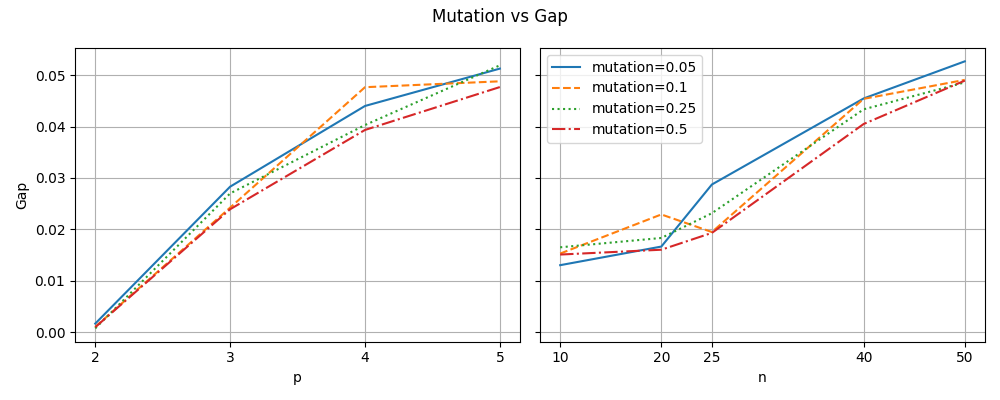
\includegraphics[width=0.9\textwidth]{figures/mutation_vs_gap.png}
  \caption{p vs. Gap and n vs. Gap based on the mutation probability}
  \label{fig:mutation_vs_gap}
\end{figure}

From this result we can see that overall the highest mutation probability ($0.5$) gets the results
closer to the optimal solution, except on the problems were either $n$ or $p$ are minimal. In these
cases the minimum mutation ($0.05$) comes on top for $n=10$ and all the mutation values get almost
the same gap for $p=2$. Outside of these minimal problems were the set of solutions is not big
enough to get an advantage from a diverse population, the lower mutation probability performs
significantly worse, specially as $n$ and $p$ increases.

\subsection{Performance searching the optimal solution\label{ss:benchmark_optimal}}

During this benchmark the algorithm was executed until the solution given by the examples
was matched. In order to attempt this multiple times with different parameters the benchmark attempts
to find the optimal solution with different combinations that will scale down in mutability and scale up
in evaluations and population, in this order.

This way the benchmark will broad the parameters of the execution in order to attempt to find the solution
if the previous combination didn't work. First, it attempts it lowering the mutation probability (using $0.5$,
$0.25$ and $0.1$ as possible values), then it attempts to allow a bigger number of maximum evaluations
($4096$, $16384$, $65536$, $262144$ and $1048576$) and finally using a bigger population ($10$, $20$, $25$,
$40$, $50$, $75$, $100$). Each advance in the number of evaluations resets the mutation to the first one,
and the same occurs when sizing up the population.

The executions that succeeded in finding the optimal can be seen in the Table \ref{tb:optimal_benchmark}.
The table shows the \emph{mutation} and \emph{population} used in the first optimal finding for that subproblem,
and it also records the number of \emph{evaluations} and the \emph{time} required in the successful 
execution, in addition to the \emph{total time} required adding the execution time of the previous attempts.
Every missing subproblem, like all those for sizes $40$ and $50$ aside of those with $p=2$, where not
resolved with the optimal solution in any of the $105$ different attempts.

\begin{table}
\caption{Results of optimal search benchmark}
\label{tb:optimal_benchmark}
\begin{center}
\begin{tabular}{|c|c|c|c|c|r|r|r|}
\hline
n & p & objective & mutation & population & evaluations & success time (ms) & total time (ms) \\
\hline
10 & 2 & 167493 & 0.50 & 10 & 182 & 3.044 & 3.044 \\
10 & 3 & 136008 & 0.50 & 10 & 1546 & 5.773 & 5.773 \\
10 & 4 & 112396 & 0.50 & 10 & 1269 & 2.851 & 2.851 \\
10 & 5 & 91105 & 0.50 & 10 & 896 & 2.013 & 2.013 \\
20 & 2 & 172817 & 0.50 & 10 & 361 & 1.409 & 1.409 \\
20 & 3 & 151533 & 0.50 & 20 & 2370 & 10.279 & 12350.606 \\
20 & 4 & 135625 & 0.50 & 10 & 11429 & 40.242 & 79.070 \\
20 & 5 & 123130 & 0.25 & 25 & 67998 & 303.726 & 31189.384 \\
25 & 2 & 175542 & 0.50 & 10 & 898 & 3.935 & 3.935 \\
25 & 3 & 155256 & 0.25 & 20 & 185100 & 805.702 & 17759.136 \\
25 & 4 & 139197 & 0.25 & 20 & 10588 & 48.033 & 15338.338 \\
25 & 5 & 123574 & 0.25 & 20 & 9380 & 42.249 & 15330.658 \\
40 & 2 & 177472 & 0.50 & 10 & 536 & 4.207 & 4.207 \\
50 & 2 & 178484 & 0.50 & 10 & 1033 & 10.694 & 10.694 \\
\hline
\end{tabular}
\end{center}
\end{table}


One of they key findings from this analysis was that only two of the subproblems resolved benefited from
the increment of evaluations over $65536$, with the $(20,5)$ barely using a couple thousand more evaluations.
This means that the current evaluation usually fails as it converges into a population no diverse enough
that fails to get closer to the optimal solution and the extra evaluations won't solve it.

A good solution for this could have been using a bigger population, specially as the problems with a
bigger $n$ will also have a lot more possible solutions. Relating the population to $n$ was followed in \ref{ss:benchmark_evaluations}.
In this case the scaling would end up reaching that value, and more, if required; but as we see only one
problem, $(20,3)$, scalated until $n=population$, with another one, the $(20,5)$, going above $n$. This
could be pointing the sweet post for $population$ below $n$,


\section{Conclusion}

The motivation of this research was offering an approach to the $p$-hub problem using GA. Implementing the 
\code{USApHMP-Q} function as the basis of the fitness function and with tailored \emph{crossover} and \emph{mutation}.

In overall terms the implemented algorithm fulfilled its objective as heuristic. With an execution below
the single second, the algorithm can generate a solution with a median gap of just $2.255\%$ over the best 
solution; ranging from half a dozen of optimal solutions found and maximum $9.619\%$ gap. With our analysis
we found the mutation probability of $0.5$ being the best performant of those tested (with a deeper analysis
we could find a better candidate in its vicinity), using that value the solution would rise to a $2.066\%$
median gap and a $8.628\%$ maximum gap.

Regarding the fit of these implementation to find the optimal solution the algorithm lacks quite a bit.
The GA accomplishes good results for the easiest subproblems, but fails to find the solution with the upper
set of subproblems. The cause of this is a set of possible solutions that outgrowns the capabilities of the
implementation. Several enchancements could be added to improve the GA in this aspect, like implementing a
selection phase evaluating more candidates, a new mutation creating more variance or a replacement that could
keep some sub-optimal but highly different solutions that could open up new paths during the crossover step.

All in all, these improvements could not be enough to close the gap enough with other approaches used in the
literature with this problem. This limitation is closely related with the foundations of the genetic algorithms
and would end up being a stone in the road sooner or later.




\bibliographystyle{IEEEtran}
\bibliography{references}

\end{document}
